% Meridian protocol v26: one-slide overview for supervisors. Overleaf: upload this file, compiler pdfLaTeX.
% Timings are the software's plan for participant 1 (lib/protocol-template.ts, renderPlan), 21 September 2026.
\documentclass[aspectratio=169,10pt]{beamer}
\usepackage[T1]{fontenc}
\usepackage{lmodern}
\usepackage{tikz}
\usepackage{array}

\setbeamertemplate{navigation symbols}{}
\setbeamersize{text margin left=0.45cm,text margin right=0.45cm}

\definecolor{ink}{HTML}{1F2A36}
\definecolor{clay}{HTML}{A8543A}
\definecolor{moss}{HTML}{3D6B45}
\definecolor{sky}{HTML}{2F5F8A}
\definecolor{amber}{HTML}{C08A1E}
\definecolor{paper}{HTML}{F6F3EE}
\definecolor{soft}{HTML}{5A6572}

\setbeamercolor{background canvas}{bg=paper}
\setbeamercolor{normal text}{fg=ink}

% A phase card: #1 colour, #2 phase name, #3 clock span, #4 minutes, #5 rows (step & time \\)
\newcommand{\card}[5]{%
  \begin{minipage}[t]{0.244\linewidth}
    \colorbox{#1}{\parbox{\dimexpr\linewidth-2\fboxsep}{\color{white}\tiny\textbf{#2}\hfill #3\ \textbar\ \textbf{#4}}}\\[-1pt]
    \tiny\setlength{\tabcolsep}{2pt}\renewcommand{\arraystretch}{0.95}%
    \begin{tabular*}{\linewidth}{@{}l@{\extracolsep{\fill}}r@{}}#5\end{tabular*}
  \end{minipage}}

% One phase on the timeline bar: #1 start min, #2 end min, #3 colour, #4 label.
\newcommand{\ph}[4]{\fill[#3] (#1,0) rectangle (#2,0.62); \node[white,align=center] at ({(#1+#2)/2},0.31) {#4};}

\begin{document}
\begin{frame}[t]
\vspace{-6pt}
{\color{ink}\large\textbf{Meridian session protocol (v26): one participant, start to finish}}\\[1pt]
{\color{soft}\scriptsize 34 steps \textbar\ \textbf{$\approx$37 min recorded} ($\approx$38 in practice) \textbar\ $\approx$67 min per participant with $\approx$30 min setup and consent}

\vspace{5pt}
\centering
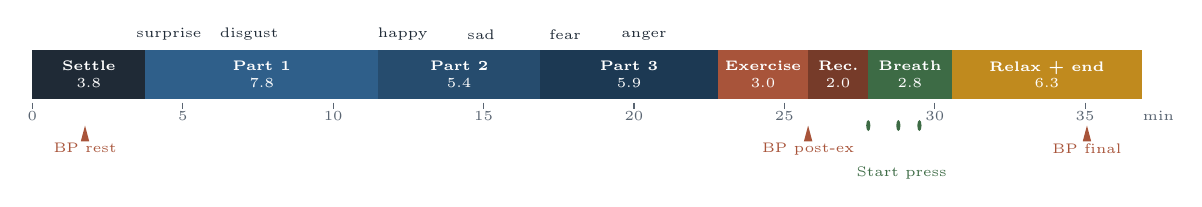
\begin{tikzpicture}[x=0.382cm,y=1cm,every node/.style={font=\tiny,inner sep=0pt}]
  % Phase bar, widths proportional to minutes (participant 1, total 36.9 min).
  \ph{0}{3.75}{ink}{\textbf{Settle}\\3.8}
  \ph{3.75}{11.5}{sky}{\textbf{Part 1}\\7.8}
  \ph{11.5}{16.88}{sky!80!black}{\textbf{Part 2}\\5.4}
  \ph{16.88}{22.79}{sky!60!black}{\textbf{Part 3}\\5.9}
  \ph{22.79}{25.79}{clay}{\textbf{Exercise}\\3.0}
  \ph{25.79}{27.79}{clay!70!black}{\textbf{Rec.}\\2.0}
  \ph{27.79}{30.56}{moss}{\textbf{Breath}\\2.8}
  \ph{30.56}{36.89}{amber}{\textbf{Relax + end}\\6.3}
  % Minute ticks
  \foreach \m in {0,5,...,35} {\draw[soft] (\m,-0.05) -- (\m,-0.13); \node[soft,anchor=north] at (\m,-0.15) {\m};}
  \node[soft,anchor=north west] at (36.9,-0.15) {min};
  % Emotion clips on the bar
  \foreach \s/\e/\n in {3.75/5.33/surprise,6.33/8.08/disgust,11.5/13.13/happy,14.13/15.71/sad,16.88/18.54/fear,19.54/21.13/anger}
    {\fill[white,opacity=0.28] (\s,0.62) rectangle (\e,0.72); \node[ink,anchor=south] at ({(\s+\e)/2},0.74) {\n};}
  % Blood pressure and Start markers
  \foreach \t/\l in {1.75/BP rest,25.79/BP post-ex,35.06/BP final}
    {\fill[clay] (\t,-0.34) -- ++(-0.14,-0.2) -- ++(0.28,0) -- cycle; \node[clay,anchor=north] at (\t,-0.56) {\l};}
  \foreach \t in {27.79,28.79,29.49} {\fill[moss] (\t,-0.34) circle (0.07);}
  \node[moss,anchor=north] at (28.9,-0.86) {Start press};
\end{tikzpicture}

\vspace{2pt}
\raggedright
\card{ink}{Getting settled}{0:00--3:45}{3.8 min}{%
  Sensor and sync check & 0:30\\
  PANAS mood (start) & 1:15\\
  Resting baseline, eyes open, BP & 2:00\\
  {\color{soft}TIPI personality: at consent} & --\\}\hfill
\card{sky}{Part 1: low HR}{3:45--11:30}{7.8 min}{%
  Clip: surprise (90 s) & 1:35\\
  Rating (SAM + emotion) & 0:40\\
  Neutral washout & 0:20\\
  Clip: disgust (100 s) & 1:45\\
  Rating & 0:40\\
  Stroop \textit{or} N-back & 1:30\\
  NASA-TLX workload & 0:45\\
  Return-to-baseline gate & $\geq$0:30\\}\hfill
\card{sky!80!black}{Part 2: mid HR}{11:30--16:53}{5.4 min}{%
  Clip: happy (93 s) & 1:38\\
  Rating & 0:40\\
  Neutral washout & 0:20\\
  Clip: sad (90 s) & 1:35\\
  Rating & 0:40\\
  Return-to-baseline gate & $\geq$0:30\\}\hfill
\card{sky!60!black}{Part 3: highest HR}{16:53--22:48}{5.9 min}{%
  Clip: fear (95 s) & 1:40\\
  Rating & 0:40\\
  Neutral washout & 0:20\\
  Clip: anger (90 s) & 1:35\\
  Rating & 0:40\\
  Word list: study + recognise & $\sim$1:00\\
  Read aloud (147 words) & $\sim$1:00\\}

\vspace{4pt}
\card{clay}{Heart-rate elevation}{22:48--25:48}{3.0 min}{%
  Stand-to-sit, as many as possible & 1:00\\
  Step-up on 20--30 cm step & 2:00\\
  {\color{soft}operator counts reps and steps} & \\}\hfill
\card{clay!70!black}{Recovery}{25:48--27:48}{2.0 min}{%
  Seated rest, BP after exertion & 2:00\\
  {\color{soft}heart-rate recovery at 1 and 2 min} & \\}\hfill
\card{moss}{Controlled breathing}{27:48--30:34}{2.8 min}{%
  Paced breathing 6/min & 1:00\\
  Paced breathing 20/min & 0:42\\
  Box breathing 4-4-4-4, 4 rounds & 1:04\\
  {\color{soft}each starts on a Start press} & \\}\hfill
\card{amber}{Relaxation and end}{30:34--36:54}{6.3 min}{%
  Guided body scan (audio) & 4:30\\
  Return to normal, final BP & 0:20\\
  PANAS mood (end) & 1:15\\
  Session complete & 0:15\\}

\vspace{5pt}
{\color{soft}\rule{\linewidth}{0.3pt}}\\[1pt]
\begin{minipage}[t]{0.33\linewidth}\tiny
\textbf{Clip order: fixed, calmest to most HR-raising.} Ranked by mean heart-rate change in a 202-study meta-analysis
(Siegel 2018): disgust $d{=}0.07$, happy 0.33, sad 0.36, fear 0.49, anger 0.52; surprise gives a brief
slow-down. Clips trimmed to 90--100\,s.
\end{minipage}\hfill
\begin{minipage}[t]{0.31\linewidth}\tiny
\textbf{One cognitive task per participant.} Stroop for participants 1--6, 13--18, \dots; N-back (0:50) for 7--12,
19--24, \dots. \textbf{Gates} wait for HR within 5 bpm and skin conductance within 10\% of baseline for 15 s.
\end{minipage}\hfill
\begin{minipage}[t]{0.33\linewidth}\tiny
\textbf{Safety:} screening skips both exercises for heart, breathing, mobility, pregnancy or ``unwell'' answers.
\textbf{Sensors:} ECG, finger PPG, skin conductance, EMG, two face cameras, thermal, Wi-Fi CSI, stereo audio.
\end{minipage}
\end{frame}
\end{document}
